\documentclass[
  10pt,
  aspectratio=169,   % 16:9 Widescreen
  %handout           % Uncomment for handout mode (no overlays)
]{beamer}

% ==============================
% Encoding & Fonts
% ==============================
\usepackage[T1]{fontenc}
\usepackage{tgheros}         % Sans-serif text font
\usepackage{newpxmath}       % Palatino-like math font
\usefonttheme{professionalfonts}
\usepackage{fix-cm}          % Flexible font sizes
\usepackage{bm}              % Bold math

% ==============================
% Theorem Environment
% ==============================
\theoremstyle{plain}
\newtheorem*{thm*}{Theorem}

% ==============================
% Tables & Layout
% ==============================
\usepackage{array}
\usepackage{varwidth}
\usepackage{multirow}
\usepackage{booktabs}
\usepackage{subcaption}
\usepackage{tikz}

% ==============================
% Bibliography
% ==============================
\usepackage[authoryear]{natbib}

% ==============================
% Beamer Settings
% ==============================
\setbeamertemplate{navigation symbols}{}
\setbeamertemplate{footline}{}
\setbeamertemplate{items}[circle]
\setbeamertemplate{blocks}[rounded][shadow=true]
\setbeamertemplate{enumerate items}[default]

\setbeamersize{text margin left=10pt, text margin right=10pt}
\setbeamerfont{itemize/enumerate subbody}{size=\normalsize}
\setbeamerfont{itemize/enumerate subsubbody}{size=\normalsize}

\useoutertheme{smoothbars}

\useoutertheme{default}
\setbeamertemplate{headline}{\vskip1.3cm}

% ==============================
% Colors (UCLA)
% ==============================
\definecolor{uclaBlue}{RGB}{39,116,174}
\definecolor{uclaRed}{RGB}{255,0,165}
\definecolor{uclaGreen}{RGB}{0,255,135}

\setbeamercolor{title}{fg=uclaBlue}
\setbeamercolor{frametitle}{fg=uclaBlue}
\setbeamercolor{structure}{fg=uclaBlue}
\setbeamercolor{block title}{fg=uclaBlue}
\setbeamercolor{item}{fg=uclaBlue}
\setbeamercolor{enumerate item}{fg=uclaBlue}
\setbeamercolor{button}{bg=uclaBlue}
\setbeamercolor{alerted text}{fg=uclaBlue}

% =====================================================================
% TITLE & AUTHOR
% =====================================================================
\title{Ownership Structure and Economic Growth}
\author{Koki Okumura}
\institute{UCLA}
\date{}

\begin{document}

\begin{frame}
  \titlepage
\end{frame}

\section{Introduction}

\begin{frame}{Ownership Structure $\Longrightarrow$ Economic Growth?}
  \label{intro} % This frame's label already exists
  \begin{itemize}
    \item Ownership structure is concentrated \hfill \hyperlink{share}{\beamerbutton{Share}}
    \begin{itemize}
      \item BlackRock, Vanguard, State Street, and Fidelity control 30\% of votes of S\&P 500 firms
      \item Top 4 chaebols account for 55\% of stock market capitalization in Korea
    \end{itemize}
    \medskip{} \pause
    \item Firms maximize shareholder values $\Longrightarrow$ \\
          Partially internalize externalities for commonly owned firm
    \medskip{} \pause
    \item Ownership structure (common ownership, cross ownership, M\&A, FDI, ...) $\Longrightarrow$ \\
          Economic growth?
    \begin{itemize}
      \item Business stealing effect
      \item Technology spillover effect
    \end{itemize}
  \end{itemize}
\end{frame}

\begin{frame}{Quantitative Schumpeterian Growth Model with Ownership Structure}
  \begin{itemize}
    \item Existing Schumpeterian growth models:
    \begin{itemize}
      \item Monopolistic competition (no strategic interaction)
      \item Very few firms in Markov perfect equilibrium
    \end{itemize}
    \medskip{}
    \item This paper: Many oligopolists
    \begin{itemize}
      \item Overlapping ownership and technology spillover across industries
    \end{itemize}
    \medskip{}\pause
    \item Quantify three inter-firm networks for publicly listed patenting firms in the US ($\simeq$ 1000 firms)
    \begin{itemize}
      \item Ownership structure
      \item Product market rivalry
      \item Technology spillover
    \end{itemize}
    \medskip{}\pause
    \item Common ownership in the US:
    \begin{itemize}
      \item Internalization of business stealing $\Longrightarrow$ $g$ $\downarrow \downarrow$
      \item Internalization of technology spillover $\Longrightarrow$ $g$ $\uparrow$
    \end{itemize}
  \end{itemize}
\end{frame}

\begin{frame}{Literature}
  \begin{itemize}
    \item Competition \& Innovation: \\
          {\footnotesize\citet{d-Aspremont1988-je,Kamien1992-la,Aghion2001-yc,Aghion2005-vw,Acemoglu2012-bj,Aghion2013-nq,Bloom2013-pn,Lopez2019-sl,Peters2020-sd,Akcigit2021-ns,Akcigit2023-zl,Liu2022-iw,Cavenaile2023-lo,Anton2023-ej,Anton2024-pw,Kini2024-kd,Hopenhayn2024-ya}}\\
          \alert{Quantitative Schumpeterian growth model with ownership structure}
    \item Hedonic Demand / Empirical IO: \\
          {\footnotesize\citet{Lancaster1966-sg,Rosen1974-ep,Berry1995-lx,Nevo2001-ja,Pellegrino2024-dn,Ederer2024-rw}}\\
          \alert{Dynamic general equilibrium / R\&D}
          %Epple1987-ru
    \item Oligopoly / Common Ownership / Market Power: \\
          {\footnotesize\citet{Rubinstein1983-pi,Rotemberg1984-jz,Neary2003-sn,Atkeson2008-zc,Gutierrez2017-wl,He2017-ix,Azar2018-cc,Azar2022-cn,Autor2020-mr,Baqaee2020-eb,De_Loecker2020-jn,Azar2021-uh,Edmond2023-bg}}
  \end{itemize}
\end{frame}

\section{Simple Model}

\begin{frame}{Simple Model}
  \begin{itemize}
    \item Static partial equilibrium model of oligopolistic competition in production and R\&D
    \begin{itemize}
      \item {\footnotesize \citet{d-Aspremont1988-je,Kamien1992-la,Leahy1997-xr,Lopez2019-sl,Anton2024-pw}} % <<< Keep citations in one line
    \end{itemize}
    \medskip{}
    \item Firm $i\in \left\{1,\ldots, n\right\}$ chooses quantity $q_i$ and R\&D effort $x_i$
    \medskip{}
    \item Linear inverse demand: $\bm{p}(\bm{q}) = \bm{b} - \bm{\Sigma} \bm{q} \quad (\bm{\Sigma} =[\sigma_{ij}]_{n \times n}, \sigma_{ii} = 1)$
    \medskip{}
    \item CRS production technology with marginal cost: $\bm{m}(\bm{x}) = \overline{\bm{m}} - \bm{\Omega} \bm{x} \quad (\bm{\Omega} =[\omega_{ij}]_{n \times n})$
    \medskip{}
    \item Quadratic R\&D cost: $c(x_i) = \frac{1}{2}x_i^2$
  \end{itemize}
\end{frame}

\begin{frame}{Common Ownership Weights}
  \label{ownership_weight}
  \begin{itemize}
    \item $\bm{K}=\left[\kappa_{ij}\right]_{n \times n}$: common ownership weights that firm $i$ places on the value of firm $j$ $\quad (\kappa_{ii} = 1)$
    \medskip{}
    \item More overlapping ownership b/w firm $i$ and $j$ $\Longrightarrow$ Higher $\kappa_{ij}$ \hfill\hyperlink{rotemberg}{\beamerbutton{Proportional Influence}}
    \medskip{}
    \item $\bm{K}=\bm{I}$: dispersed ownership (each firm maximizes its own value)
    \medskip{}
    \item $\bm{K}=\bm{1}_{n \times n}$: monopoly (maximizes total producer surplus)
  \end{itemize}
\end{frame}

\begin{frame}{Cournot \& R\&D Game}
  \begin{itemize}
    \item Firm $i$'s profit:
    \begin{align*}
      \pi_{i}(\bm{q}, \bm{x}) & = [p_i(\bm{q}) - m_i(\bm{x})]q_{i}  - c(x_i) \\
                             & = \left[ b_{i} - \sum_{j=1}^{n} \sigma_{ij} q_{j} - \overline{m}_{i} + \sum_{j=1}^{n} \omega_{ij} x_{j} \right]q_{i} - \frac{1}{2}x_{i}^{2}
    \end{align*}
    \item Given $\left\{ q_{j}, x_{j}\right\} _{j\neq i}$, firm $i$ chooses $q_{i}$ and $x_{i}$ to maximize $\sum_{j}\kappa_{ij}\pi_{j}(\bm{q}, \bm{x})$
  \end{itemize}
\end{frame}

\begin{frame}{Impact of Common Ownership on R\&D}
  \begin{itemize}
    \item Comparative statics where $\left\{ q_{k}, x_{k}\right\} _{k\neq i}$ are held constant:
    \[
      \frac{\partial x_{i}}{\partial\kappa_{ij}} = \frac{q_j}{2 - \omega_{ii}^2}( 2\textcolor{uclaRed}{\omega_{ij}} - \omega_{ii} \textcolor{uclaBlue}{\sigma_{ij}}) \quad\quad  \forall \ j \neq i
    \]
    \begin{itemize}
      \item SOC: $2>\omega_{ii}^2$
    \end{itemize}
    \medskip{}
    \item Internalize \alert{business stealing effect}: $\partial^2 x_{i}/\partial\kappa_{ij}\partial\textcolor{uclaBlue}{\sigma_{ij}}<0$
    \medskip{}
    \item Internalize \textcolor{uclaRed}{technology spillover effect}: $\partial^2 x_{i}/\partial\kappa_{ij}\partial\textcolor{uclaRed}{\omega_{ij}}>0$
  \end{itemize}
\end{frame}

\begin{frame}{Preview of Identification Strategy}
  \label{identification_overview} % <<< ラベルを追加
  \begin{center}
    \renewcommand{\arraystretch}{1.5} % 行間を広げる (1.0がデフォルト)
    \begin{tabular}{lV{\linewidth}}
      Networks                              & Measurement\tabularnewline
      \hline\hline
      Common ownership $\bm{K}$         & Institutional investor holdings \citep{Backus2021-yt} \tabularnewline
      \hline
      Product market rivalry $\bm{\Sigma}$ & Product proximity \citep{Hoberg2016-jm}: \tabularnewline
                                          & Text analysis of business description \tabularnewline
      \hline
      Technology spillover $\bm{\Omega}$   & Technological proximity \citep{Jaffe1986-yz,Bloom2013-pn}: \tabularnewline
                                          & Patent classification\tabularnewline
    \end{tabular}
    \renewcommand{\arraystretch}{1.0} % デフォルトに戻す
  \end{center}
\end{frame}

\section{Growth Model}
\begin{frame}{Schumpeterian Growth Model}
  \begin{itemize}
    \item Linear quadratic aggregator (final good):
    \[
      Y_{t}=\bm{q}_{t}^{T}\bm{b}_{t}-\frac{1}{2}\bm{q}_{t}^{T}\bm{\Sigma}\bm{q}_{t}
    \]
    \item Linear inverse demand:
    \[
      \bm{p}_{t}=\bm{b}_{t}-\bm{\Sigma}\bm{q}_{t}
    \]
    \item CRS production technology (intermediate good): \[q_{i,t}=a_{i,t}l_{i,t}\]
    \item Each firm has knowledge capital (state variable): $z_{i,t}$
    \medskip{}
    \item Each firm allocates knowledge capital to improve labor productivity and product quality:
    \[
      \zeta a_{i,t}+b_{i,t}=z_{i,t}
    \]
  \end{itemize}
\end{frame}

\begin{frame}{Law of Motion of Knowledge Capital}
  \[
    d\bm{z}_{t}=\left(\underbrace{\bm{\Omega}\bm{z}_{t}}_{\text{tech spillover}}+\underbrace{\mu\bm{x}_{t}}_{\text{R\&D}}\right)dt+\underbrace{\gamma\bm{z}_{t} \circ d\bm{W}_{t}}_{\text{shocks}}
  \]
  \begin{itemize}
    \item $\bm{\Omega}=\left[\omega_{ij}\right]$: technology spillover matrix
    \medskip{}
    \item $x_{i,t}=\sqrt{d_{i,t}}$
    \begin{itemize}
      \item $d_{i,t}$: R\&D input in terms of final good
      \item Innovation elasticity is 0.5
      \medskip{}
    \end{itemize}
    \item $\mu$, $\gamma$: positive scalars
  \end{itemize}
\end{frame}

\begin{frame}{Market Clearing and Preference}
  \begin{itemize}
    \item Inelastic labor supply:
    \[
      L=\sum_{i}l_{i,t}
    \]
    \item Final good market clearing:
    \[
      C_{t}+\underbrace{\sum_{i}d_{i,t}}_{\text{R\&D input}}=Y_{t}
    \]
    \item Risk neutral representative household:
    \[
      \max\ \bm{E}_{t}\left[\int_{t}^{\infty}\exp\left(-\rho s\right)C_{s}ds\right]
    \]
  \end{itemize}
\end{frame}

\section{Equilibrium}

\begin{frame}{Cournot-Nash Equilibrium}
  \label{cournot}
  \begin{itemize}
    \item Firm $i$'s gross profit before subtracting dynamic R\&D cost: \hyperlink{diagram}{\beamerbutton{Diagram}}
    \begin{align*}
      \pi_{i,t} & =p_{i,t}q_{i,t}-w_{t}l_{i,t}=\left(b_{i,t}-\sum_{j}\sigma_{ij}q_{j,t}-\frac{w_{t}}{a_{i,t}}\right)q_{i,t}\quad\text{where}\quad\zeta a_{i,t}+b_{i,t}=z_{i,t}
    \end{align*}
    \item Given $w_{t}$, $z_{i,t}$, and $\left\{ q_{j,t}\right\} _{j\neq i}$, firm $i$ chooses $a_{i,t}$, $b_{i,t}$, and $q_{i,t}$ to maximize $\sum_{j}\kappa_{ij}\pi_{j,t}$
    \pause\medskip{}
    \item Quantity is a linear function of knowledge capital:
    \[
      \bm{q}(\bm{z}_{t})=\left\{ \underbrace{2\frac{\zeta}{L}\bm{1}_{n \times n}}_{\text{labor cost}}+\underbrace{\bm{\Sigma}}_{\text{substitutability}}+\underbrace{\bm{K}\circ\bm{\Sigma}}_{\text{ownership}\times\text{substitutability}}\right\} ^{-1}\bm{z}_{t}
    \]
    \item Ownership-weighted gross profits are expressed in quadratic form: $\sum_{j}\kappa_{ij}\pi_{j,t}=\bm{z}_{t}^{T}\bm{Q}^{i}\bm{z}_{t}$ \hyperlink{Q}{\beamerbutton{Q}}
  \end{itemize}
\end{frame}

\begin{frame}{Linear-Quadratic Differential Game}
  \begin{itemize}
    \item Given other firms' R\&D $\left\{ x_{j,t}\right\} _{j\neq i,t\geq0}$, firm $i$ chooses R\&D $\left\{ x_{i,t}\right\} _{t\geq0}$ to maximize
    \[
      \max_{\left\{ x_{i,t}\right\} _{t\geq0}}\quad V^{i}\left(\text{\ensuremath{\bm{z}}}_{0}\right)\equiv\bm{E}_{0}\left[\int_{0}^{\infty}\exp\left(-\rho t\right)\left\{ \sum_{j}\kappa_{ij}\left(\pi_{j,t}-x_{j,t}^{2}\right)\right\} dt\right]
    \]
    subject to $d\bm{z}_{t}=\left(\bm{\Omega}\bm{z}_{t}+\mu\bm{x}_{t}\right)dt+\gamma\bm{z}_{t} \circ d\bm{W}_{t}$
    \pause\medskip{}
    \item Firm $i$'s HJB equation:
    \[
      \rho V^{i}\left(\bm{z}\right)=\max_{x_{i}}\left\{ \bm{z}^{T}\bm{Q}^{i}\bm{z}-\sum_{j}\kappa_{ij}x_{j}^{2}+V_{\bm{z}}^{i}\left(\bm{z}\right)\left[\bm{\Omega}\bm{z}+\mu\bm{x}\right]+\frac{\gamma^{2}}{2}\bm{z}^{T}V_{\bm{zz}}^{i}\left(\bm{z}\right)\bm{z}\right\}
    \]
  \end{itemize}
\end{frame}

\begin{frame}{HJB Equations $\Longrightarrow$ Riccati Equations}
  \label{hjb}
  \begin{itemize}
    \item Guess and verify $V^{i}\left(\bm{z}\right)=\bm{z}^{T}\bm{X}^{i}\bm{z}$ (for any $\bm{z}$)
    \medskip{}
    \item $\bm{X}^{i}$ is the solution of stacked algebraic Riccati equations \hyperlink{riccati}{\beamerbutton{Riccati}}
    \medskip{}
    \item All public patenting firms in the US in our dataset $\simeq$1000 firms $\Longrightarrow$ \\
          $1000^{3}=1$ billion undetermined coefficients (20 seconds on my laptop)
    \medskip{}
  \end{itemize}
  \begin{center}
    \begin{tabular}{@{}p{5cm}ccc@{}}
      \toprule
      Oligopolistic Schumpeterian           & Computation time & \# of firms    & Productivity space \\
      \midrule
      \citet{Cavenaile2023-lo}              & $O(2^n)$         & 4              & 6 grid       \\
      Our model                             & $O(n^4)$         & $\approx$1000  & Continuous         \\
      \bottomrule
    \end{tabular}
  \end{center}
\end{frame}

\begin{frame}{Balanced Growth Path}
  \begin{itemize}
    \item R\&D strategy: $x_{i,t}=\left(\mu \bm{X}_{i}^{i}\right)^{T}\bm{z}_{t}$ where $\bm{X}_{i}^{i}$ is the $i$ th column of $\bm{X}^{i}$
    \item The law of motion is rewritten as $d\bm{z}_{t}=\alert{\bm{\Phi}}\bm{z}_{t}dt+\gamma\bm{z}_{t} \circ d\bm{W}_{t}$ where
    \[
      \alert{\bm{\Phi}}\equiv\underbrace{\bm{\Omega}}_{\text{Tech Spillover}}+\underbrace{\mu^{2}\left[\bm{X}_{1}^{1} \ \cdots \ \bm{X}_{n}^{n}\right]^{T}}_{\text{R\&D}}
    \]
    \vspace{-5mm}
  \end{itemize}
  \begin{thm*}
    Consider the deterministic economy $(\gamma=0)$. If \alert{$\bm{\Phi}$} is irreducible, then:

    (i) There exists the largest positive eigenvalue of \alert{$\bm{\Phi}$}, $g$, and associated positive eigenvector, $\bm{z}^{*}$.

    (ii) There exists a globally stable BGP such that the knowledge capital growth rate of all firms is $g$, and the knowledge capital distribution is a scalar multiple of $\bm{z}^{*}$.
  \end{thm*}
  \begin{itemize}
    \item Proof: Perron--Frobenius Theorem
    \item ``\alert{$\bm{\Phi}$} is irreducible'' $\Longleftrightarrow$ ``All firms are directly or indirectly connected technologically''
  \end{itemize}
\end{frame}

\begin{frame}{Intuition of Why the Model Has the BGP}
  \begin{itemize}
    \item On the BGP, \alert{$\bm{a}_{t}$}, ${\color{uclaBlue}\bm{b}_{t}}$, \alert{$\bm{z}_{t}$}, and ${\color{uclaBlue}\bm{q}_{t}}$ grow at the same rate
  \end{itemize}
  \begin{center}
    \renewcommand{\arraystretch}{1.3}  % Increases the row height by 30%
    \begin{tabular}{>{\raggedright\arraybackslash}p{5cm}>{\raggedright\arraybackslash}p{6cm}}
      Technological Choice: & $\zeta{\color{uclaBlue}a_{i,t}}+{\color{uclaBlue}b_{i,t}}={\color{uclaBlue}z_{i,t}}$ \\
      Linear Production Technology: & ${\color{uclaBlue}q_{i,t}}={\color{uclaBlue}a_{i,t}}l_{i,t}$ \\
      Inelastic Labor Supply: & $L=\sum_{i}l_{i,t}$ \\
    \end{tabular}
    \renewcommand{\arraystretch}{1.0}  % Reset to default spacing
  \end{center}
  \begin{itemize}
    \item Linear and quadratic term in $\color{uclaBlue}\bm{q}_{t}$ of output grow at the same rate: \hyperlink{summary}{\beamerbutton{Equilibrium Summary}}
    \[
      Y_{t}={\color{uclaBlue}\bm{q}_{t}^{T}\bm{b}_{t}}-\frac{1}{2}{\color{uclaBlue}\bm{q}_{t}^{T}}\bm{\Sigma}{\color{uclaBlue}\bm{q}_{t}}
    \]
  \end{itemize}
\end{frame}

\begin{frame}{Partial Equilibrium Diagram and BGP}
  \label{diagram}
  \begin{minipage}{0.45\textwidth}
    \centering
    \begin{tikzpicture}[scale=0.7]
      \pgfmathsetmacro{\b}{3}
      \pgfmathsetmacro{\c}{1}
      \pgfmathsetmacro{\qeq}{(\b - \c)/2}
      % Axes
      \draw[->] (0,0) -- (6,0) node[right] {$q_i$};
      \draw[->] (0,0) -- (0,5) node[above] {$p_i$};
      % Equilibrium price line
      \draw[dashed] (0,{\b-\qeq}) -- (\qeq,{\b-\qeq});
      \node[left] at (0,{\b-\qeq}) {$p_i^*$};
      % Residual demand and marginal revenue
      \draw[thick,blue] (0,\b) -- (\b,0) node[below] {};
      \draw[thick,dotted,blue!70!black] (0,\b) -- ({\b/2},0); % MR
      % Marginal cost
      \draw[thick,dashed,red] (0,\c) -- (5.5,\c);
      \node[left] at (0,\b) {$b_i-\sum_{j\neq i} \sigma_{ij} q_j$};
      \node[left] at (0,\c) {$w/a_i$};
      % Equilibrium quantity
      \draw[dashed] (\qeq,0) -- (\qeq,\b-\qeq);
      \node[below] at (\qeq,0) {$q_i^*$};
    \end{tikzpicture}
  \end{minipage}%
  \begin{minipage}{0.45\textwidth}
    \centering
    \begin{tikzpicture}[scale=0.7]
      \pgfmathsetmacro{\b}{3*1.5}
      \pgfmathsetmacro{\c}{1*1.5}
      \pgfmathsetmacro{\qeq}{(\b - \c)/2}
      % Axes
      \draw[->] (0,0) -- (6,0) node[right] {$q_i$};
      \draw[->] (0,0) -- (0,5) node[above] {$p_i$};
      % Residual demand and marginal revenue
      \draw[thick,blue] (0,\b) -- (\b,0);
      \draw[thick,dotted,blue!70!black] (0,\b) -- ({\b/2},0); % MR
      % Equilibrium price line
      \draw[dashed] (0,{\b-\qeq}) -- (\qeq,{\b-\qeq});
      \node[left]  at (0,{\b-\qeq}) {$(1+g)p_i^*$};
      % Marginal cost
      \draw[thick,dashed,red] (0,\c) -- (5.5,\c);
      \node[left] at (0,\b) {$(1+g)(b_i-\sum_{j\neq i} \sigma_{ij} q_j)$};
      \node[left] at (0,\c) {$(1+g)w/a_i$};
      % Equilibrium quantity
      \draw[dashed] (\qeq,0) -- (\qeq,\b-\qeq);
      \node[below] at (\qeq,0) {$(1+g)q_i^{*}$};
    \end{tikzpicture}
  \end{minipage}
  \begin{itemize}
    \item $a_i$, $b_i$, $q_i(=a_i l_i)$, $p_i$, and $w/a_i$ grow at the same rate of $g$
    \item (i) (consumer surplus / producer surplus) and (ii) (cost / revenue) stay the same
  \end{itemize} \hyperlink{cournot}{\beamerbutton{Back}}
\end{frame}

\begin{frame}{Expected Growth Rate and Utility}
  \label{aggregation}
  \begin{itemize}
    \item Apply Itô's lemma:\hfill \hyperlink{Y_process}{\beamerbutton{Decomposition}}
    \[
    \begin{array}{cl}
      \log Y_{t} & =\log\left(\bm{z}_{t}^{T}\bm{Q}\bm{z}_{t}\right)\\
      d\bm{z}_{t} & =\bm{\Phi}\bm{z}_{t}dt+\gamma\bm{z}_{t} \circ d\bm{W}_{t}
    \end{array}
    \Longrightarrow \quad \bm{E}_{t}\left[\left.g_{t}\right|\bm{z}_{t}\right]
    \]
    \item Expected utility is expressed in quadratic form: \hfill \hyperlink{X}{\beamerbutton{X}}
    \[
      \bm{E}_{t}\left[\left.\int_{t}^{\infty}\exp\left(-\rho s\right)C_{s}ds\right|\bm{z}_{t}\right]=\bm{z}_{t}^{T}X\bm{z}_{t}
    \]
    \item Solve the equilibrium once $\Longrightarrow$ Can compute expected growth and utility for any $\bm{z}_{t}$
  \end{itemize}
\end{frame}

\section{Identification}

\begin{frame}{Common Ownership Weight $\bm{K}$}
  \begin{itemize}
    \item \citet{Backus2021-yt} construct a dataset on investors' holdings based on Form 13F
    \item Baseline: \citet{Rotemberg1984-jz} proportional influence \hfill\hyperlink{rotemberg}{\beamerbutton{Proportional Influence}}
  \end{itemize}
  \begin{center}
    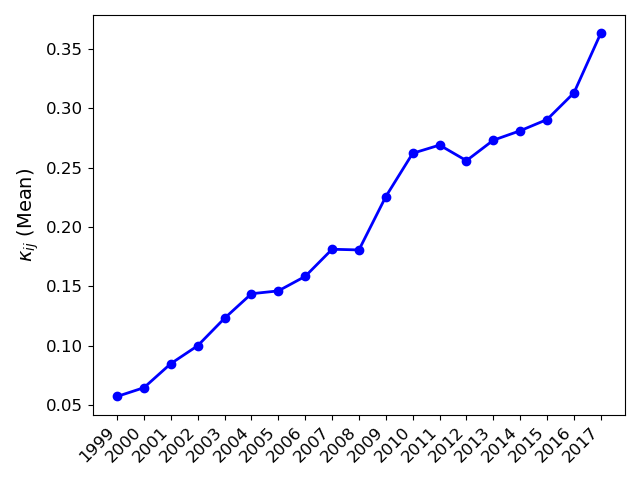
\includegraphics[width=7cm]{figures/kappa}
  \end{center}
\end{frame}

\begin{frame}{Product Market Rivalry $\bm{\Sigma}$}
  \label{product_identification}
  \begin{itemize}
    \item \citet{Hoberg2016-jm} estimates product proximity using business descriptions in 10-K
    \medskip{}
    \item \citet{Pellegrino2024-dn} estimates $\alpha$ to align with the cross-price elasticity of demand \hyperlink{micro_vs_ghl}{\beamerbutton{micro estimates}}
  \end{itemize}
  \medskip{}
  \[
    \underbrace{\sigma_{ij}}_{\text{substitutability}}=\alpha\times\text{product proximity b/w }i\text{ and }j\quad\left(i\neq j\right)
  \]
\end{frame}

\begin{frame}{Technological Proximity $\widetilde{\bm{\Omega}}$}
  \begin{itemize}
    \item Technological profile of firm $i$
    \begin{itemize}
      \item The vector of the share of patents held by firm $i$ in each technology class
      \item Baseline: group-level patent classifications ($\approx4000$)
      \medskip{}
    \end{itemize}
    \medskip{}
    \item \citet{Jaffe1986-yz} technological proximity measure $\tilde{\omega}_{ij}$:
    \begin{itemize}
      \item Cosine similarity of the technological profiles b/w firm $i$ and $j$
    \end{itemize}
  \end{itemize}
\end{frame}

\begin{frame}{Distribution of Knowledge Capital $\bm{z}_t$}
  \begin{table}[htbp]
    \centering
    \begin{tabular}{cl}
      \toprule
      Variables & Identification \\
      \midrule
      $\pi_{i,t}$
      & Gross profit (before R\&D cost)
      $=$ Revenue $-$ Cost of goods sold \\[6pt]
      $\bm{q}_t$
      &
      $\pi_{i,t}=\displaystyle\sum_{j}\kappa_{ij}\,\sigma_{ij}\,q_{i,t}\,q_{j,t}$ \\[6pt]
      $\zeta/L$
      & Matches sample firms' cost share (average markup) \\[6pt]
      $\bm{z}_t$
      &
      $\displaystyle \bm{z}_{t}
      =\left\{2\frac{\zeta}{L}\bm{J}+\bm{\Sigma}+\bm{K}\circ\bm{\Sigma}\right\}\bm{q}_{t}$ \\
      \bottomrule
    \end{tabular}
  \end{table}
\end{frame}

\begin{frame}{Technology Spillover $\bm{\Omega}=\beta\times$Technological Proximity $\bm{\widetilde{\Omega}}$ \hyperlink{first_stage}{\beamerbutton{First Stage}}}
  \label{regression}
  {\footnotesize
  \vspace{-5mm}
  \[
    z_{i,t+1}-z_{i,t}
    =\beta\sum_{j\neq i}\tilde{\omega}_{ij,t}z_{j,t}
    +\text{Year FE}_{t}
    +\epsilon_{i,t}
  \]
  \begin{center}
    \setlength{\tabcolsep}{6pt} % Adjust column spacing
    \begin{tabular}{lccc}
      \hline\hline
      & (1) & (2) & (3) \\
      & $z_{i,t+1}-z_{i,t}$
      & $z_{i,t+1}-z_{i,t}$
      & $z_{i,t+1}-z_{i,t}$ \\
      \hline
      $\sum_{j\neq i}\tilde{\omega}_{ij,t}z_{j,t}$
      & $\begin{array}{c}\text{0.000191}^{***}\\(\text{0.000035})\end{array}$
      & $\begin{array}{c}\text{0.000152}^{***}\\(\text{0.000035})\end{array}$
      & $\begin{array}{c}\text{0.000140}^{***}\\(\text{0.000039})\end{array}$ \\
      $\sqrt{\text{R\&D Expenditure}}$
      &
      & $\begin{array}{c}\text{0.037}^{**}\\(\text{0.021})\end{array}$
      &  \\
      \hline
      Year Fixed Effects                & $\checkmark$ & $\checkmark$ & $\checkmark$ \\
      IV                                &              &              & $\checkmark$ \\
      IV 1st Stage F-statistics         &              &              & 4176         \\
      No.\ observations                 & 16,324       & 15,173       & 14,181       \\
      \hline\hline
    \end{tabular}
  \end{center}
  SEs clustered by years and 4-digit NAICS industries are reported in parentheses.
  {*} $p<\text{0.1}$, {**} $p<\text{0.05}$, {***} $p<\text{0.01}$.}
  \begin{itemize}
    \item IV: Firm-specific tax price of R\&D from federal and state-specific rules \citep{Bloom2013-pn}
  \end{itemize}
\end{frame}

\begin{frame}{Identification: Summary}
  \begin{itemize}
    \item Publicly available data + Compustat
  \end{itemize}
  \begin{table}[h]
    \centering
    \small % フォントサイズを小さくする
    \begin{tabular}{llll}
      \toprule
      Notation                           & Description                                      & Value   & Source                                   \\
      \midrule
      $\bm{\Sigma}$                   & Product proximity                                &         & Form 10-K, \citet{Hoberg2016-jm}          \\
      $\bm{\widetilde{\Omega}}$       & Technological proximity                          &         & USPTO, Patent classification             \\
      $\bm{K}$                        & Common ownership weights                         &         & Form 13-F, \citet{Backus2021-yt}          \\
      $\alpha$                           & Product proximity $\rightarrow$ Substitutability & 0.12    & \citet{Pellegrino2024-dn}                \\
      $\beta$                            & Technological proximity $\rightarrow$ Spillover  & 0.00014 & Estimate the law of motion               \\
      $\gamma$                           & Std. of idiosyncratic shocks                    & 0.027   & Estimate the law of motion               \\
      $\zeta/L$                          & Labor augmentation efficiency                    & 0.0063  & Compustat, Cost of goods sold            \\
      $\rho$                             & Discount rate                                    & 0.10    & $>$ risk free rates, $<$ private R\&D returns \\
      $\mu$                              & R\&D efficiency                                  & 0.05    & 1.7\% economic growth rate               \\
      \bottomrule
    \end{tabular}
  \end{table}
\end{frame}

\begin{frame}{Fit b/w Model and Data}
  \begin{itemize}
    \item Comparison of firm-level model-generated values ($x$-axis) with observed data ($y$-axis)
  \end{itemize}
  \medskip{}
  \begin{center}
    \begin{figure}
      \centering
      \setcounter{subfigure}{0}
      \subfloat[Log of Profit (Targeted)]{\begin{centering}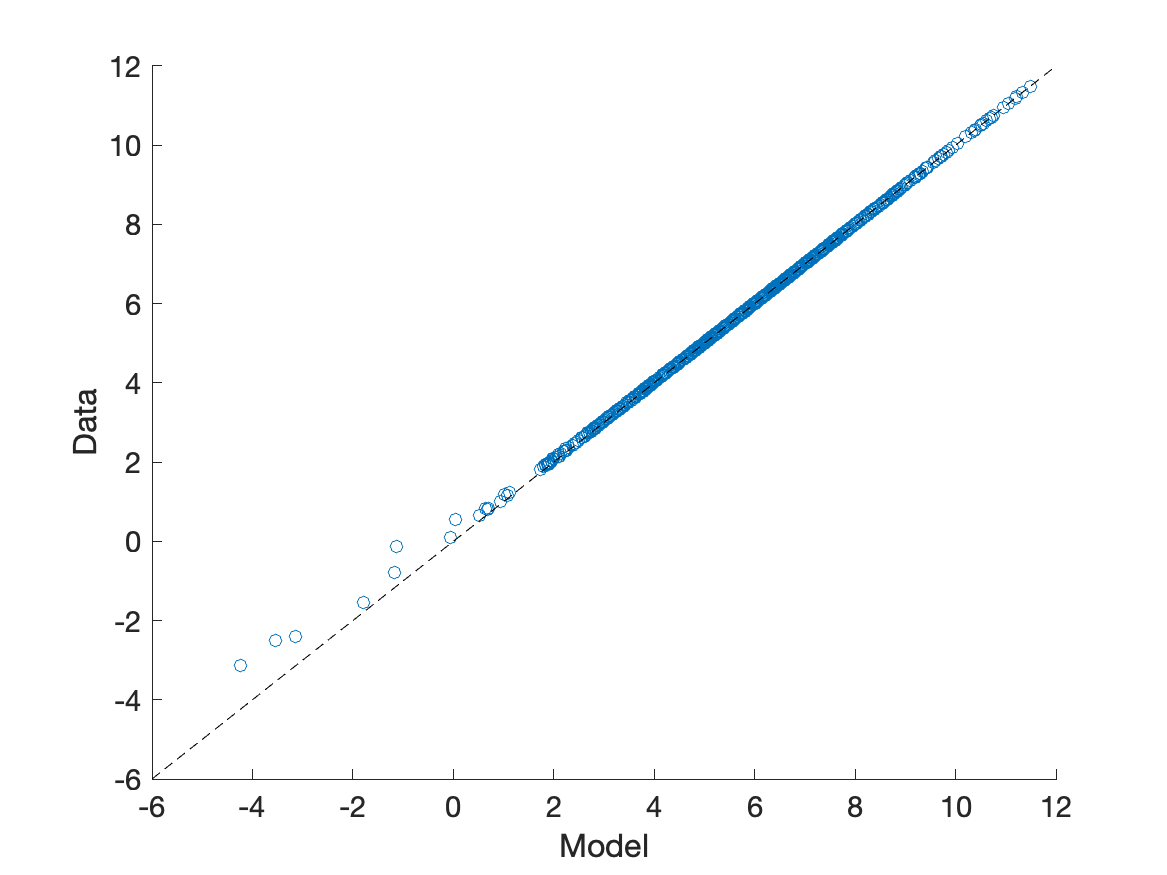
\includegraphics[width=4.5cm]{figures/OO_profit_vs_data}\par\end{centering}}
      \subfloat[Log of Sales]{\begin{centering}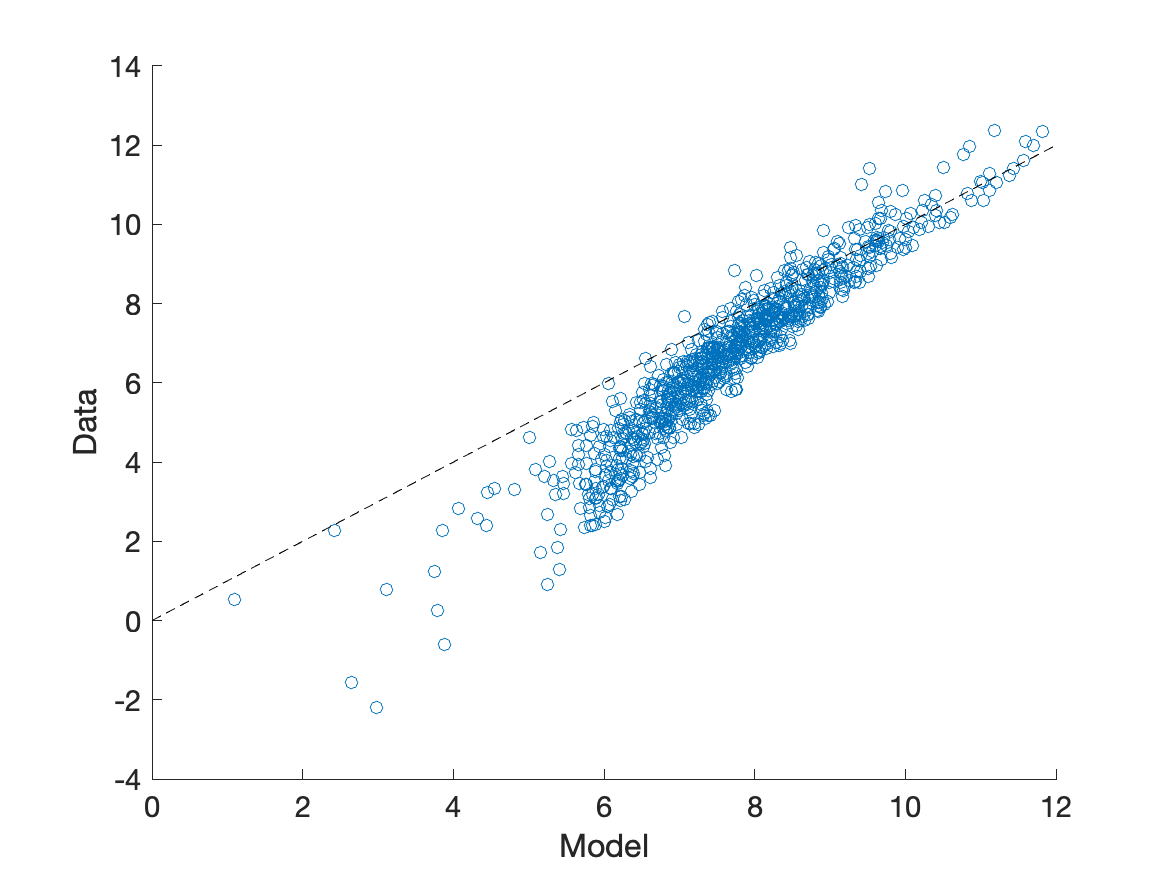
\includegraphics[width=4.5cm]{figures/OO_sales_vs_data}\par\end{centering}}
      \subfloat[Log of R\&D Expenditure]{\begin{centering}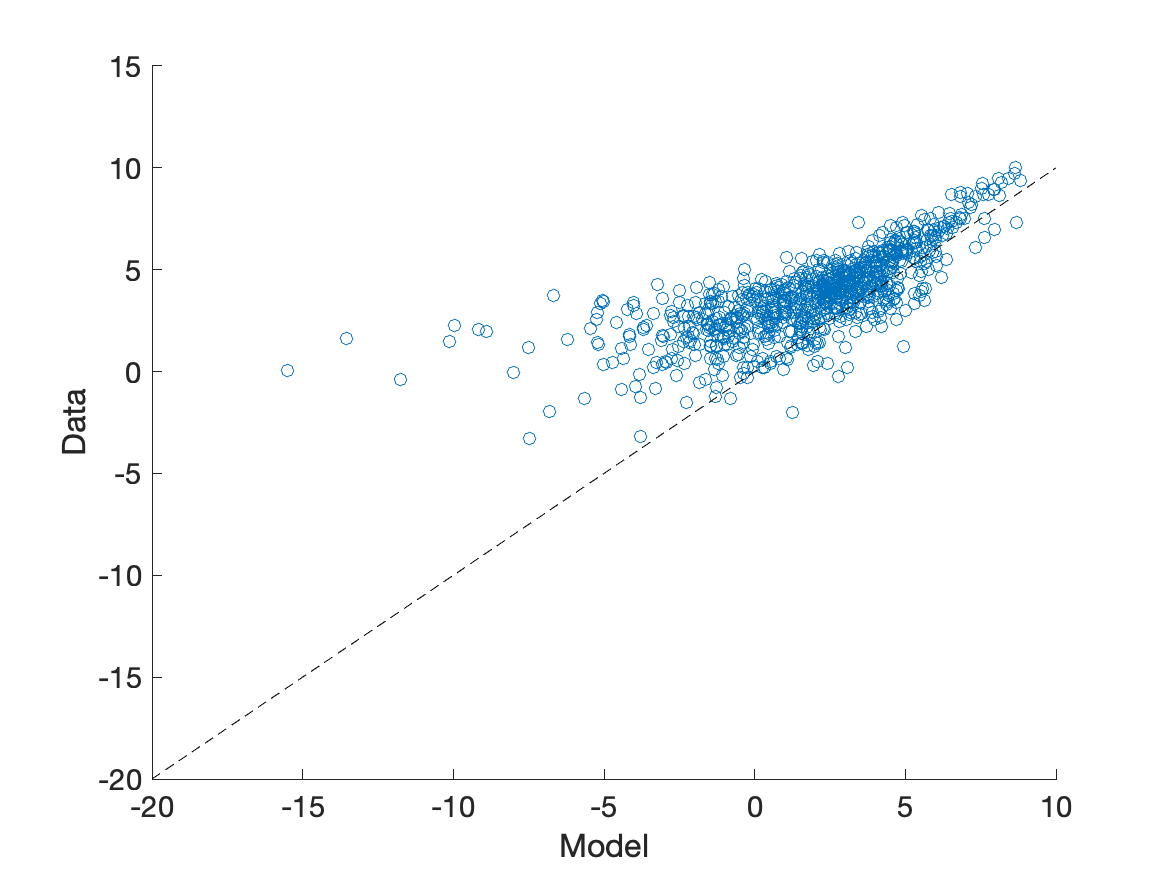
\includegraphics[width=4.5cm]{figures/OO_r_and_d_vs_data}\par\end{centering}}
    \end{figure}
  \end{center}
\end{frame}

\section{Exercise}

\begin{frame}{Counterfactual Ownership Structures}
  \begin{table}[h]
    \centering
    \renewcommand{\arraystretch}{1.5} % 行間を広げる
    \begin{tabular}{ll}
      \toprule
      Ownership Structure & Description \\
      \midrule
      Baseline            & Observed ownership structure in 2017 \\
      Dispersed           & $\bm{K}^D=\bm{I}$ \\
      Mean$=$1999         & $\kappa_{ij,2017}^{M1999}=\text{const}\times\kappa_{ij,2017}$ and $\bm{E}\left[\kappa_{ij,2017}^{M1999}\right]=\bm{E}\left[\kappa_{ij,1999}\right]$ for $j\neq i$\\
      Uniform             & $\kappa_{ij,2017}^U=\bm{E}\left[\kappa_{ij, 2017}\right]$ for $j\neq i$ \\
      Monopoly            & $\bm{K}^M=\bm{1}$ \\
      \bottomrule
    \end{tabular}
    \renewcommand{\arraystretch}{1.0} % デフォルトに戻す
  \end{table}
\end{frame}

\begin{frame}{Total Output}
  \centering
  \setlength{\tabcolsep}{3pt}
  \begin{tabular}{@{} c *{5}{c} @{}}
    \toprule
    \multirow{2}{*}{\shortstack[t]{Total Output in 2017 \\ (Social Optimum: 100)}}
    & \multicolumn{5}{c}{Ownership (Baseline: 2017)} \\
    \cmidrule(lr){2-6}
    & Dispersed
    & Mean$=$1999
    & Uniform
    & Baseline
    & Monopoly \\
    \midrule
    Baseline
    & 91.30 & 91.02 & 90.78 & 89.08 & 89.17 \\
    \midrule
    \shortstack[t]{Only Business Steal \\ $\bm{\Omega}=[0]$}
    & \visible<2->{91.30}
    & \visible<2->{91.02}
    & \visible<2->{90.78}
    & \visible<2->{89.08}
    & \visible<2->{89.17} \\
    \midrule
    \shortstack[t]{Only Tech Spill \\ $\bm{\Sigma}=\bm{I},\,\zeta/L=0$}
    & \visible<3->{75.00}
    & \visible<3->{75.00}
    & \visible<3->{75.00}
    & \visible<3->{75.00}
    & \visible<3->{75.00} \\
    \bottomrule
  \end{tabular}
  \medskip{}
  \begin{itemize}
    \item Inelastic labor supply $\Longrightarrow$ Changes arise from product misallocation
    \item Common ownership exacerbates product misallocation
  \end{itemize}
\end{frame}

\begin{frame}{Total R\&D Expenditure}
  \centering
  \setlength{\tabcolsep}{3pt}
  \begin{tabular}{@{} c *{5}{c} @{}}
    \toprule
    \multirow{2}{*}{\shortstack[t]{Total R\&D in 2017 \\ (Social Optimum: 100)}}
    & \multicolumn{5}{c}{Ownership (Baseline: 2017)} \\
    \cmidrule(lr){2-6}
    & Dispersed
    & Mean$=$1999
    & Uniform
    & Baseline
    & Monopoly \\
    \midrule
    Baseline
    & 27.08 & 26.83 & 26.44 & 23.21 & 18.48 \\
    \midrule
    \shortstack[t]{Only Business Steal \\ $\bm{\Omega}=[0]$}
    & \visible<2->{29.08}
    & \visible<2->{28.72}
    & \visible<2->{27.95}
    & \visible<2->{24.23}
    & \visible<2->{18.85} \\
    \midrule
    \shortstack[t]{Only Tech Spill \\ $\bm{\Sigma}=\bm{I},\,\zeta/L=0$}
    & \visible<3->{18.27}
    & \visible<3->{18.34}
    & \visible<3->{18.75}
    & \visible<3->{18.86}
    & \visible<3->{19.84} \\
    \bottomrule
  \end{tabular}
  \medskip{}
  \begin{itemize}
    \item Internalization of business stealing $>$ Internalization of technology spillover
    \item Network heterogeneity is important
  \end{itemize}
\end{frame}

\begin{frame}{Expected Growth Rate}
  \centering
  \setlength{\tabcolsep}{3pt}
  \begin{tabular}{@{} c *{5}{c} @{}}
    \toprule
    \multirow{2}{*}{\shortstack[t]{Expected Economic \\ Growth Rate in 2017 (\%)}}
    & \multicolumn{5}{c}{Ownership (Baseline: 2017)} \\
    \cmidrule(lr){2-6}
    & Dispersed
    & Mean$=$1999
    & Uniform
    & Baseline
    & Monopoly \\
    \midrule
    Baseline
    & 1.796 & 1.793 & 1.791 & 1.753 & 1.713 \\
    \midrule
    \shortstack[t]{Only Business Steal \\ $\bm{\Omega}=[0]$}
    & \visible<2->{1.097}
    & \visible<2->{1.094}
    & \visible<2->{1.093}
    & \visible<2->{1.062}
    & \visible<2->{1.020} \\
    \midrule
    \shortstack[t]{Only Tech Spill \\ $\bm{\Sigma}=\bm{I},\,\zeta/L=0$}
    & \visible<3->{2.051}
    & \visible<3->{2.054}
    & \visible<3->{2.068}
    & \visible<3->{2.072}
    & \visible<3->{2.107} \\
    \bottomrule
  \end{tabular}
  \medskip{}
  \begin{itemize}
    \item In baseline, the expected growth rate is
    \begin{itemize}
      \item 0.043 pp (2.4\%) lower compared to dispersed ownership, and
      \item 0.040 pp (2.2\%) lower compared to common ownership level in 1999.
    \end{itemize}
  \end{itemize}
\end{frame}

\begin{frame}{Expected Social Welfare}
  \centering
  \setlength{\tabcolsep}{3pt}
  \begin{tabular}{@{} c *{5}{c} @{}}
    \toprule
    \multirow{2}{*}{\shortstack[t]{Expected Social Welfare \\ (Social Optimum: 100)}}
    & \multicolumn{5}{c}{Ownership (Baseline: 2017)} \\
    \cmidrule(lr){2-6}
    & Dispersed
    & Mean$=$1999
    & Uniform
    & Baseline
    & Monopoly \\
    \midrule
    Baseline
    & 87.72 & 87.42 & 87.16 & 85.25 & 85.18 \\
    \midrule
    \shortstack[t]{Only Business Steal \\ $\bm{\Omega}=[0]$}
    & \visible<2->{88.83}
    & \visible<2->{88.53}
    & \visible<2->{88.30}
    & \visible<2->{86.44}
    & \visible<2->{86.41} \\
    \midrule
    \shortstack[t]{Only Tech Spill \\ $\bm{\Sigma}=\bm{I},\,\zeta/L=0$}
    & \visible<3->{68.81}
    & \visible<3->{68.82}
    & \visible<3->{68.88}
    & \visible<3->{68.89}
    & \visible<3->{69.02} \\
    \bottomrule
  \end{tabular}
  \medskip{}
  \begin{itemize}
    \item In the baseline, the consumption-equivalent welfare loss is
    \begin{itemize}
      \item 2.8\% compared to dispersed ownership, and
      \item 2.5\% compared to the common ownership level in 1999.
    \end{itemize}
  \end{itemize}
\end{frame}

%begin{frame}{Ownership Concentration and Aggregate R\&D}
% \begin{itemize}
%   \item When
%         \begin{itemize}
%           \item Ownership concentration reduces aggregate R\&D, and
%           \item Appropriability effect is strong enough,
%         \end{itemize}
%         \medskip{}
% \end{itemize}
% \centering
% \begin{tikzpicture}[>=stealth, font=\normalsize]
%   % x軸の描画
%   \draw[->] (0,0) -- (11,0) node[right]{\large Aggregate R\&D};
%
%   % ラベルノードの配置(文字を折り返すためtext widthとalignを指定)
%   \node[below, text width=2cm, align=center] at (1,-0.2) {Monopoly};
%   \node[below, text width=3cm, align=center] at (4,-0.2) {Firms maximize\\ profit};
%   \node[below, text width=2.5cm, align=center] at (7,-0.2) {Social\\optimum};
%   \node[below, text width=3cm, align=center] at (10,-0.2) {Firms capture \\total surplus};
%
%   % 各ラベルの上(x座標はノードと同じ位置、y座標0.5)に丸点を配置
%   \foreach \x in {1,4,7,10} {
%       \fill[black] (\x,0) circle (2pt);
%     }
%
%   % 左側の矢印(Monopoly~Firms maximize total profit)
%   \draw[<-, thick] (1,0.5) -- (4,0.5) node[midway, above=8pt]{Ownership concentration};
%
%   % 右側の矢印(Social Optimum~Firms maximize total surplus)
%   \draw[<-, thick] (7,0.5) -- (10,0.5) node[midway, above=8pt]{Ownership concentration};
%
% \end{tikzpicture}
%end{frame}

\begin{frame}{Firm Value Share}
  \centering
  \setlength{\tabcolsep}{3pt}
  \begin{tabular}{@{} c *{5}{c} @{}}
    \toprule
    \multirow{2}{*}{\shortstack[t]{Firm Value \\ Share in 2017 (\%)}}
    & \multicolumn{5}{c}{Ownership (Baseline: 2017)} \\
    \cmidrule(lr){2-6}
    & Dispersed
    & Mean$=$1999
    & Uniform
    & Baseline
    & Monopoly \\
    \midrule
    Baseline
    & 28.74  & 29.63  & 33.43 & 33.34 & 40.92 \\
    \midrule
    \shortstack[t]{Only Business Steal \\ $\bm{\Omega}=[0]$}
    & \visible<2->{27.91}
    & \visible<2->{28.80}
    & \visible<2->{32.60}
    & \visible<2->{33.51}
    & \visible<2->{40.14} \\
    \midrule
    \shortstack[t]{Only Tech Spill \\ $\bm{\Sigma}=\bm{I},\,\zeta/L=0$}
    & \visible<3->{64.82}
    & \visible<3->{64.81}
    & \visible<3->{64.76}
    & \visible<3->{64.74}
    & \visible<3->{64.63} \\
    \bottomrule
  \end{tabular}
  \medskip{}
  \begin{itemize}
    \item In baseline, firm value share is
    \begin{itemize}
      \item 5.6\% lower compared to dispersed ownership, and
      \item 4.7\% lower compared to common ownership level in 1999.
    \end{itemize}
  \end{itemize}
\end{frame}

\begin{frame}{When Common Ownership Affects only R\&D Decisions}
  \begin{itemize}
    \item Common ownership only influences R\&D decisions (cf. \cite{d-Aspremont1988-je})
  \end{itemize}
  \begin{center}
    \setlength{\tabcolsep}{3pt}
    \begin{tabular}{@{}lccc@{}}
      \toprule
      & \multicolumn{3}{c}{Ownership Structure} \\
      \cmidrule(lr){2-4}
      & Dispersed
      & {\color{uclaBlue}Common R\&D}
      & Baseline \\
      \midrule
      \shortstack[l]{Output (Social Optimum: 100)}
      & 91.30 & {\color{uclaBlue}91.30} & 89.08 \\
      \shortstack[l]{R\&D Expenditure (Social Optimum: 100)}
      & 26.17 & {\color{uclaBlue}19.76} & 22.36 \\
      \shortstack[l]{Expected Growth Rate (\%)}
      & 1.796 & {\color{uclaBlue}1.726} & 1.753 \\
      \shortstack[l]{Expected Social Welfare (Social Optimum: 100)}
      & 87.72 & {\color{uclaBlue}87.49} & 85.25 \\
      \shortstack[l]{Firm Value Share (\%)}
      & 28.74 & {\color{uclaBlue}29.04} & 34.34 \\
      \bottomrule
    \end{tabular}
  \end{center}
  \begin{itemize}
    \item Lowest R\&D expenditure and expected growth rate
    \item Intermediate social welfare and firm value share
  \end{itemize}
\end{frame}

\begin{frame}{Optimal Uniform R\&D Subsidy \hyperlink{optimal}{\beamerbutton{Social Optimum}}}
  \begin{center}
    \begin{figure}
      \centering
      \setcounter{subfigure}{0}
      \subfloat[Expected Growth]{\begin{centering}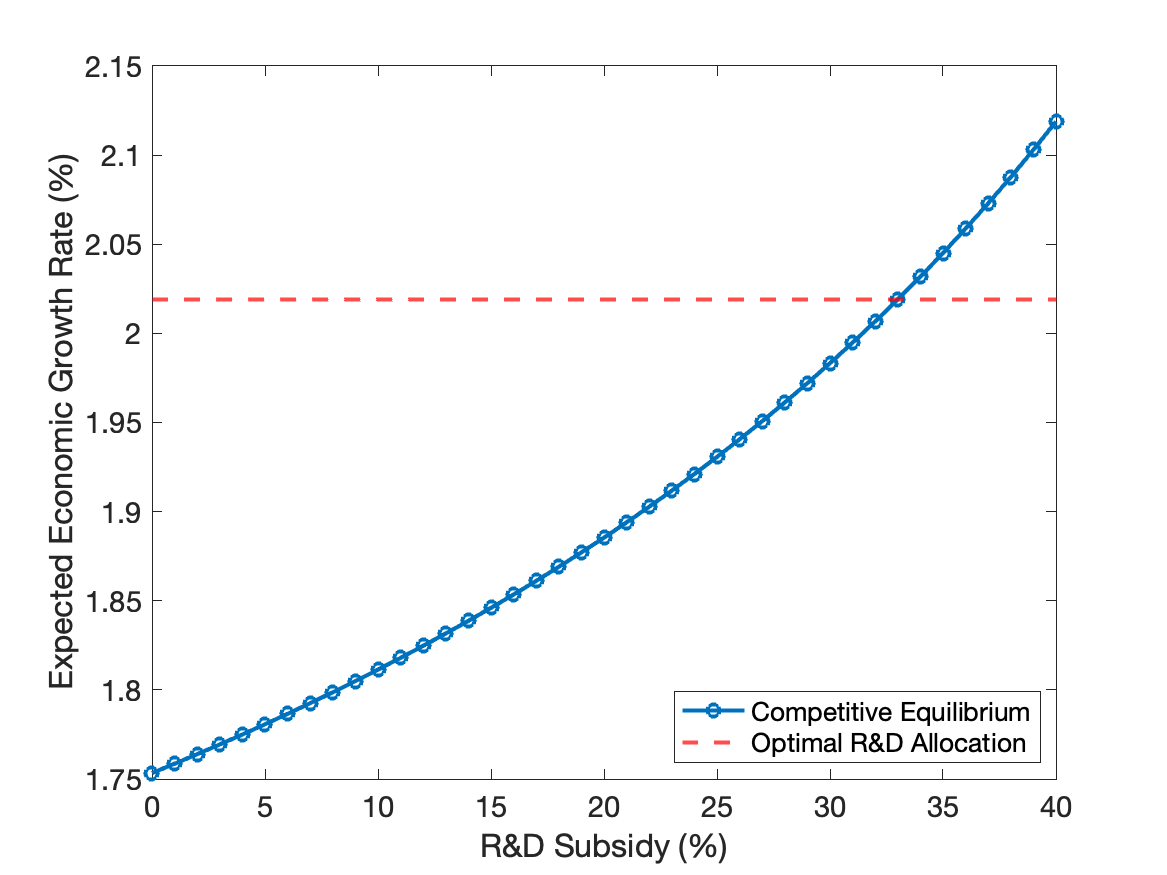
\includegraphics[width=6cm]{figures/subsidy_growth}\par\end{centering}}
      \subfloat[Expected Social Welfare]{\begin{centering}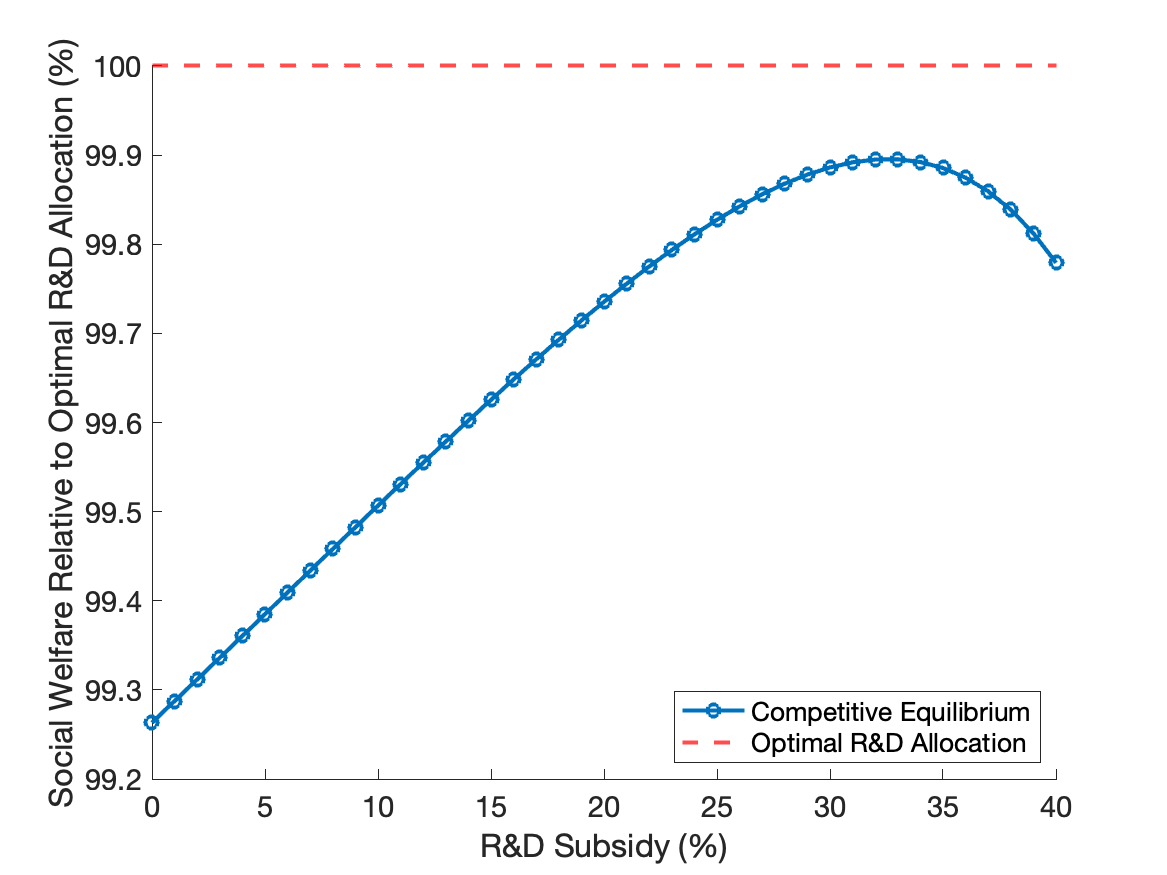
\includegraphics[width=6cm]{figures/subsidy_welfare}\par\end{centering}}
    \end{figure}
  \end{center}
  \begin{itemize}
    \item Optimal rate is $s=$33\%, which increases $g$ by 0.25 pp (14\%)
    %\item CE Welfare loss relative to optimal R\&D allocation is reduced to 0.1\% (Initially 0.7\%)
  \end{itemize}
\end{frame}

\section{Conclusion}
\begin{frame}{Conclusion}
  \begin{itemize}
    \item Quantitative Schumpeterian growth model with ownership structure
    \begin{itemize}
      \item Utilize micro data and computational capability
    \end{itemize}
    \medskip{}
    \item Common ownership in the US:
    \begin{enumerate}
      \item Internalization of business stealing effect $\Longrightarrow$ $g$ $\downarrow$$\downarrow$
      \item Internalization of technology spillover effect $\Longrightarrow$ $g$ $\uparrow$
    \end{enumerate}
    \medskip{}
    \item Potential applications:
    \begin{itemize}
      \item Chaebols in Korea
      \item Zaibatsu (pre-WWII) and cross-shareholding (late 20th century) in Japan
      \item FDI / multinational companies and international technology diffusion
      \item Technology licensing
    \end{itemize}
  \end{itemize}
\end{frame}

\appendix
\section{Appendix}

\begin{frame}{Share of Top 5 Shareholders in Largest Market Cap Firms \hyperlink{intro}{\beamerbutton{Back}}}
  \label{share}
  % --- 1行目 ---
  \begin{minipage}[t]{0.3\textwidth} % 1番目: Microsoft
    \centering
    \footnotesize % <--- \scriptsize から変更
    \begin{tabular}{lr}
      \toprule
      Microsoft                      &        \\
      \midrule
      \alert{Vanguard}     & 9.20\% \\
      \alert{Blackrock}    & 7.75\% \\
      Steven Ballmer                 & 4.48\% \\
      \alert{State Street} & 3.97\% \\
      \alert{Fidelity}     & 2.66\% \\
      \bottomrule
    \end{tabular}
  \end{minipage}
  \hfill % スペース
  \begin{minipage}[t]{0.3\textwidth} % 2番目: Nvidia
    \centering
    \footnotesize % <--- \scriptsize から変更
    \begin{tabular}{lr}
      \toprule
      Nvidia                         &        \\
      \midrule
      \alert{Vanguard}     & 8.93\% \\
      \alert{BlackRock}    & 7.74\% \\
      \alert{Fidelity}     & 4.12\% \\
      \alert{State Street} & 3.97\% \\
      Jensen Huang                   & 3.80\% \\
      \bottomrule
    \end{tabular}
  \end{minipage}
  \hfill % スペース
  \begin{minipage}[t]{0.3\textwidth} % 3番目: Apple
    \centering
    \footnotesize % <--- \scriptsize から変更
    \begin{tabular}{lr}
      \toprule
      Apple                          &        \\
      \midrule
      \alert{Vanguard}     & 9.29\% \\
      \alert{Blackrock}    & 7.48\% \\
      \alert{State Street} & 3.96\% \\
      \alert{Fidelity}     & 2.27\% \\
      Geode Capital                  & 2.26\% \\
      \bottomrule
    \end{tabular}
  \end{minipage}

  \vspace{0.5cm} % 行間の垂直スペース

  % --- 2行目 ---
  \begin{minipage}[t]{0.3\textwidth} % 4番目: Google
    \centering
    \footnotesize % <--- \scriptsize から変更
    \begin{tabular}{lr}
      \toprule
      Google                         &        \\
      \midrule
      \alert{Vanguard}     & 7.36\% \\
      \alert{Blackrock}    & 6.47\% \\
      \alert{State Street} & 3.39\% \\
      \alert{Fidelity}     & 3.01\% \\
      Sergey Brin                    & 2.99\% \\
      \bottomrule
    \end{tabular}
  \end{minipage}
  \hfill % スペース
  \begin{minipage}[t]{0.3\textwidth} % 5番目: Amazon
    \centering
    \footnotesize % <--- \scriptsize から変更
    \begin{tabular}{lr}
      \toprule
      Amazon                         &        \\
      \midrule
      Jeffrey Bezos                  & 8.58\% \\
      \alert{Vanguard}     & 7.77\% \\
      \alert{Blackrock}    & 6.50\% \\
      \alert{State Street} & 3.44\% \\
      \alert{Fidelity}     & 3.10\% \\
      \bottomrule
    \end{tabular}
  \end{minipage}
  \hfill % スペース
  \begin{minipage}[t]{0.3\textwidth} % 6番目: Meta
    \centering
    \footnotesize % <--- \scriptsize から変更
    \begin{tabular}{lr}
      \toprule
      Meta                           &        \\
      \midrule
      \alert{Vanguard}     & 7.55\% \\
      \alert{Blackrock}    & 6.50\% \\
      \alert{Fidelity}     & 5.38\% \\
      Accel IX LP                    & 3.88\% \\
      \alert{State Street} & 3.40\% \\
      \bottomrule
    \end{tabular}
  \end{minipage}
\end{frame}

\begin{frame}{Equity Investments by Big Tech in AI Startups \hyperlink{intro}{\beamerbutton{Back}}}
  \label{ai}
  \begin{table}[ht]
    \centering
    \begin{tabular}{@{}lccc@{}}
      \toprule
      Shareholding percentage & Microsoft & Google & Amazon \\
      \midrule
      OpenAI (ChatGPT) &
      49\% &
      — &
      — \\
      Anthropic (Claude) &
      — &
      14\% &
      23\% \\
      \bottomrule
    \end{tabular}
  \end{table}
\end{frame}

\begin{frame}{Technology \& Product Proximity: Example}
  % --- Use columns environment for side-by-side content ---
  \begin{columns}[T] % [T] aligns content at the top
    % --- Left Column ---
    \begin{column}{0.45\textwidth} % Adjust width as needed
      \centering % Center the content within the column
      \begin{tabular}{lr}
        \toprule
        Tesla vs. Ford       &      \\
        \midrule
        Technology Proximity & 0.11 \\
        Product Proximity    & 0.15 \\ % Note the % sign
        \bottomrule
      \end{tabular}
    \end{column}
    % --- Right Column ---
    \begin{column}{0.45\textwidth} % Adjust width as needed
      \centering % Center the content within the column
      \begin{tabular}{lr}
        \toprule
        Apple vs. Intel      &      \\
        \midrule
        Technology Proximity & 0.57 \\
        Product Proximity    & 0.00 \\ % Note: No % sign here
        \bottomrule
      \end{tabular}
    \end{column}
  \end{columns}
\end{frame}

\begin{frame}{\cite{Rotemberg1984-jz} Proportional Influence}
  \label{rotemberg}
  \begin{itemize}
    \item $o\in\left\{ 1,2,...,n_{o}\right\} $: owners
    \item $s_{io}$: the proportion of shares in firm $i$ owned by owner $o$ where $\sum_{o}s_{io}=1$
    \item $\widehat{V}_{i}$: value of firm $i$
    \item $\widetilde{V}_{o}\equiv\sum_{i}s_{io}\widehat{V}_{i}$: value of owner $o$
    \item Firms' objective:
    \[
      \sum_{o}s_{io}\widetilde{V}_{o}\propto\sum_{j}\kappa_{ij}\widehat{V}_{j}
    \]
    where
    \[
      \kappa_{ij}\equiv\frac{\bm{s}_{i}^{T}\bm{s}_{j}}{\bm{s}_{i}^{T}\bm{s}_{i}} = \cos\left( \bm{s}_{i}, \bm{s}_{j} \right)\sqrt{\frac{IHHI_j}{IHHI_i}}
      \quad \text{where} \quad \bm{s}_{i}\equiv\left[s_{i1},...,s_{io},...,s_{in_{o}}\right]^{T}
    \]
  \end{itemize}
  \vfill % ボタンを下に配置するためのスペース
  \hfill\hyperlink{ownership_weight}{\beamerbutton{Back}} % <<< 2ページ目(intro)へのボタンを追加 (右寄せ)
\end{frame}

\begin{frame}{Total Surplus}
  \begin{itemize}
    \item Total surplus for product $i$:
    \[
      ts_{i}(\bm{q},\bm{x}) = \pi_{i}(\bm{q}, \bm{x}) +  cs_{i}(\bm{q})= q_{i} \left[ b_{i} - \textcolor{uclaRed}{\frac{1}{2}}\sum_{j=1}^{n} \sigma_{ij} q_{j} - \overline{m}_{i} + \sum_{j=1}^{n} \omega_{ij} x_{j} \right] - \frac{1}{2}x_{i}^{2}
    \]
  \end{itemize}
\end{frame}

\begin{frame}{R\&D Externalities}
  \label{rd_externalities} % <--- この行を追加
  \begin{enumerate}
    \item Business stealing effect
    \begin{itemize}
      \item Innovators steel the business (profits) of other firms
    \end{itemize}
    \medskip{}
    \item Technology spillover effect
    \begin{itemize}
      \item Innovation improves the productivity of other firms
    \end{itemize}
    \medskip{}
    \item Appropriability effect (market power)
    \begin{itemize}
      \item Innovators cannot appropriate the entire consumer surplus
    \end{itemize}
  \end{enumerate}
\end{frame}

\begin{frame}{R\&D Allocation and Externalities}
  \label{rd_allocation} % <--- この行を追加
  \begin{itemize}
    \item Firms maximize common owner weighted profits:
    \[
      \bm{x}^* = (\textcolor{uclaRed}{\bm{K}\circ\bm{\Omega}}) [\bm{\Sigma}+\alert{\bm{K} \circ \bm{\Sigma}} - \bm{\Omega}(\textcolor{uclaRed}{\bm{K}\circ\bm{\Omega}})]^{-1} (\bm{b} - \overline{\bm{m}})
    \]
    \item Firms maximize common owner weighted total surplus ($\star$):
    \[
      \bm{x}^*_{TS} = (\textcolor{uclaRed}{\bm{K}\circ\bm{\Omega}}) \left[ \textcolor{uclaGreen}{\frac{1}{2}} (\bm{\Sigma} + \alert{\bm{K} \circ \bm{\Sigma}}) - \bm{\Omega} (\textcolor{uclaRed}{\bm{K}\circ\bm{\Omega}}) \right]^{-1} (\bm{b} - \overline{\bm{m}})
    \]
    \item $\bm{K}=\bm{1}_{n \times n}$ in ($\star$) $\Longrightarrow$ Social Optimum
    \medskip{}
    \item Externalities: (i) \textcolor{uclaGreen}{Appropriability}, (ii) \alert{Business stealing}, (iii) \textcolor{uclaRed}{Technology spillover}
  \end{itemize}
\end{frame}

\begin{frame}{Generalized Hedonic-Linear Demand \citep{Pellegrino2024-dn}}
  \label{ghl}
  \begin{itemize}
    \item $i\in\left\{ 1,2,...,n\right\} $: firms / products
    \item 1 unit of product $i$ provides
    \begin{itemize}
      \item 1 unit of idiosyncratic characteristic $k\in\left\{ 1,2,...,n\right\} $
      \item ${\color{uclaBlue}\psi{}_{k,i}}$ unit of shared characteristic $k\in\left\{ n+1,n+2,...,n+n_{k}\right\} $ where $\sum_{k}{\color{uclaBlue}\psi_{k,i}^{2}}=1$
    \end{itemize}
    \item Aggregate each characteristic:
    \[
      y_{k,t}=\begin{cases}
        q_{k,t}                                   & k=1,2,...,n           \\
        \sum_{i}{\color{uclaBlue}\psi{}_{k,i}}q_{i,t} & k=n+1,n+2,...,n+n_{k}
      \end{cases}
    \]
    \item Linear quadratic aggregator over characteristics:
    \[
      Y_{t}=\left(1-\alpha\right)\sum_{k=1}^{n}\left(\underbrace{\hat{b}_{k,t}y_{k,t}-\frac{1}{2}y_{k,t}^{2}}_{\text{idiosyncratic characteristic}}\right)+\alpha\sum_{k=n+1}^{n+n_{k}}\left(\underbrace{\hat{b}_{k,t}y_{k,t}-\frac{1}{2}y_{k,t}^{2}}_{\text{shared characteristic}}\right)
    \]
  \end{itemize}
\end{frame}

% \begin{frame}{Product Substitutability $\propto$ Product Proximity \citep{Pellegrino2024-dn}}
%  \begin{itemize}
%    \item $\Sigma=\left[\sigma_{ij}\right]$ is estimated using product proximity measure
%    \item Product proximity is based on text analysis of product description in 10k filings
%          \[
%            \sigma_{ij}=\alpha\times\text{product cosine similarity b/w }i\text{ and }j\quad\left(i\neq j\right)
%          \]
%  \end{itemize}
%  \begin{center}
%    \begin{tikzpicture}[scale=3.5]
%      % Define the coordinates for the unit circle
%      \draw[domain=0:90] plot ({cos(\x)}, {sin(\x)});
%      % Axes
%      \draw[->] (0, 0) -- (1.2, 0) node[right] {Characteristic 1};
%      \draw[->] (0, 0) -- (0, 1.2) node[above] {Characteristic 2};
%      % Points
%      \coordinate (a1) at (0.8, 0.6);
%      \coordinate (a2) at (0.3, 0.95);
%      % Labels for points
%      \fill[black] (a1) circle (0.5pt) node[right] {$ \ \text{Product 1}$};
%      \fill[black] (a2) circle (0.5pt) node[right] {$ \ \ \text{Product 2}$};
%      % Connecting lines
%      \draw[dashed] (0, 0) -- (a1);
%      \draw[dashed] (0, 0) -- (a2);
%      % Angle arc
%      \node at (0.1, 0.15) {$\theta$};
%    \end{tikzpicture}
%  \end{center}
% \end{frame}

\begin{frame}{Generalized Hedonic-Linear Demand \citep{Pellegrino2024-dn}}
  \begin{itemize}
    \item Quality:
    \[
      b_{i}=\left(1-\alpha\right)\hat{b}_{i}+\alpha\sum_{k=n+1}^{n+n_{k}}\psi_{k}\hat{b}_{k}
    \]
    \item Inverse demand:
    \[
      \frac{\bm{p}}{P}=\bm{b}-\bm{\Sigma}\bm{q}
    \]
    \item Inverse cross price elasticity of demand:
    \[
      \frac{\partial\log p_{i}}{\partial\log q_{j}}=-\frac{q_{j}}{p_{i}}\cdot\sigma_{ij}
    \]
    \item Cross price elasticity of demand:
    \[
      \frac{\partial\log q_{i}}{\partial\log p_{j}}=-\frac{p_{j}}{q_{i}}(\bm{\Sigma}^{-1})_{ij}
    \]
  \end{itemize}
\end{frame}

\begin{frame}{Static Profits}
  \label{Q}
  \begin{itemize}
    \item Gross profit: $\pi_{i,t}=\sum_{j}\kappa_{ij}\sigma_{ij}q_{i,t}q_{j,t}$
    \item Firms choose labor productivity and product quality: $\zeta a_{i,t}=\sqrt{\zeta w_{t}}$, $b_{i,t}=z_{i,t}-\sqrt{\zeta w_{t}}$
    \item Labor market clearing: $L=\sum_{i}\frac{q_{i,t}}{a_{i,t}}$ $\Longrightarrow$$\sqrt{\zeta w_{t}}=\frac{\zeta}{L}\sum_{i}q_{i,t}$
    \item $\bm{q}_{t}=\bm{N}\bm{z}_{t}$ where $N\equiv\left\{ 2\frac{\zeta}{L}\bm{J}+\bm{\Sigma}+\bm{K}\circ\bm{\Sigma}\right\} ^{-1}$
    \item $\bm{N}_{i}$: the $i$ th row of $\bm{N}$
    \item Ownership weighted profit:
    {\small
    \[
      \sum_{j}\kappa_{ij}\frac{\pi_{j,t}}{P_{t}}=\sum_{j}\kappa_{ij}\sum_{h}\kappa_{jh}\sigma_{jh}q_{j,t}q_{h,t}=\bm{z}_{t}^{T}\bm{Q}^{i}\bm{z}_{t}
    \]}
    where
    {\small
    \[
      \bm{Q}^{i}=\frac{1}{2}\sum_{j}\kappa_{ij}\sum_{h}\kappa_{jh}\sigma_{jh}\left(N_{j}^{T}N_{h}+N_{h}^{T}N_{j}\right)
    \]}
    \hyperlink{cournot}{\beamerbutton{Back}}
  \end{itemize}
\end{frame}

\begin{frame}{Riccati Equations}
  \label{riccati}
  \begin{itemize}
    \item $V^{i}\left(\bm{z}\right)=\bm{z}^{T}\bm{X}^{i}\bm{z}$ where $\bm{X}^{i}$ is the solution of the stacked Riccati equation
    {\small
    \[
      0=\bm{Q}^{i}-\mu^{2}\sum_{j}\kappa_{ij}\bm{X}_{j}^{j}\left(\bm{X}_{j}^{j}\right)^{T}+\left(\bm{\Phi}-\frac{1}{2}\left(\rho-\gamma^{2}\right)\bm{I}\right)^{T}\bm{X}^{i}+\bm{X}^{i}\left(\bm{\Phi}-\frac{1}{2}\left(\rho-\gamma^{2}\right)\bm{I}\right)
    \]}
    \begin{itemize}
      \item $\bm{X}_{i}^{i}\equiv$ the $i$ th column of $\bm{X}^{i}$
      \item $\bm{\Phi}\equiv\bm{\Omega}+\mu^{2}\left[\begin{array}{ccc}\bm{X}_{1}^{1} & \cdots & \bm{X}_{n}^{n}\end{array}\right]^{T}$
    \end{itemize}
    \medskip{}
    \item Algorithm: Given $\left[\begin{array}{ccc}\bm{X}_{\tau}^{1} & \cdots & \bm{X}_{\tau}^{n}\end{array}\right]$, update $\left[\begin{array}{ccc}\bm{X}_{\tau-\Delta}^{1} & \cdots & \bm{X}_{\tau-\Delta}^{n}\end{array}\right]$ by
    {\small
    \[
      -\frac{\bm{X}_{\tau}^{i}-\bm{X}_{\tau-\Delta}^{i}}{\Delta}=\bm{Q}^{i}-\mu^{2}\sum_{j}\kappa_{ij}\bm{X}_{j,\tau}^{j}\left(\bm{X}_{j,\tau}^{j}\right)^{T}+\left(\bm{\Phi}_{\tau}-\frac{1}{2}\left(\rho-\gamma^{2}\right)\bm{I}\right)^{T}\bm{X}_{\tau}^{i}+\bm{X}_{\tau}^{i}\left(\bm{\Phi}_{\tau}-\frac{1}{2}\left(\rho-\gamma^{2}\right)I\right)
    \]}
  \end{itemize}
  \hyperlink{hjb}{\beamerbutton{Back}}
\end{frame}

\begin{frame}{Summary of Equilibrium}
  \label{summary}
  \begin{center}
    \begin{tabular}{ll}
      Description                     & Expression\tabularnewline
      \hline
      Production strategy             & $\bm{q}_{t}=N\bm{z}_{t}$\tabularnewline
      R\&D strategy                   & $\bm{x}_{t}=\mu\tilde{X}\bm{z}_{t}$\tabularnewline
      Law of motion                   & $d\bm{z}_{t}=\left(\Omega\bm{z}_{t}+\mu\bm{x}_{t}\right)dt+\gamma\bm{z}_{t}dW_{t}$\tabularnewline
      Profit of final producers       & $\Pi_{t}^{F}/P_{t}=\bm{q}_{t}^{T}\left(\frac{1}{2}\Sigma\right)\bm{q}_{t}$\tabularnewline
      Total operating profit of firms & $\Pi_{t}/P_{t}=\bm{q}_{t}^{T}\left(\frac{1}{2}\Sigma\circ\left(K+K^{T}\right)\right)\bm{q}_{t}$\tabularnewline
      Labor income                    & $w_{t}L/P_{t}=\bm{q}_{t}^{T}\left(\frac{\zeta}{L}J\right)\bm{q}_{t}$\tabularnewline
      Output                          & $Y_{t}=\bm{q}_{t}^{T}\left(\frac{\zeta}{L}J+\frac{1}{2}\Sigma+\frac{1}{2}\Sigma\circ\left(K+K^{T}\right)\right)\bm{q}_{t}$\tabularnewline
      Consumption                     & $C_{t}=Y_{t}-\bm{x}_{t}^{T}\bm{x}_{t}$\tabularnewline
    \end{tabular}
  \end{center}
  \hyperlink{aggregation}{\beamerbutton{Back}}
\end{frame}

\begin{frame}{Output and Expected Utility}
  \label{X}
  \begin{itemize}
    \item Output: $Y_{t}=\bm{q}_{t}^{T}Q\bm{q}_{t}$ where
    \[
      Q=\frac{\zeta}{L}J+\frac{1}{2}\Sigma+\frac{1}{2}\Sigma\circ\left(K+K^{T}\right)
    \]
    \item Expected utility:
    \[
      V\left(\bm{z}_{t}\right)\equiv\bm{E}_{t}\left[\left.\int_{t}^{\infty}\exp\left(-\rho s\right)C_{s}ds\right|\bm{z}_{t}\right]=\bm{z}_{t}^{T}X\bm{z}_{t}
    \]
    where $X$ is the solution of the Lyapunov equation (obtained from households' HJB equation):
    \[
      0=Q-\mu^{2}\tilde{X}^{T}\tilde{X}+X\left(\Phi-\frac{1}{2}\left(\rho-\gamma^{2}\right)I\right)+\left(\Phi-\frac{1}{2}\left(\rho-\gamma^{2}\right)I\right)^{T}X
    \]
  \end{itemize}
  \hyperlink{aggregation}{\beamerbutton{Back}}
\end{frame}

\begin{frame}{Social Optimum}
  \label{optimal}
  \begin{itemize}
    \item Static optimal allocation: $\bm{q}_{t}^{*}=N^{*}\bm{z}_{t}\quad\text{where}\quad N^{*}\equiv\left\{ 2\frac{\zeta}{L}J+\Sigma\right\} ^{-1}$
    \item Optimal output: $Y_{t}^{*}=\bm{z}_{t}^{T}Q^{*}\bm{z}_{t}$ where $Q^{*}=\frac{1}{2}N^{*}$
    \item Optimal expected utility:
    \[
      V^{*}\left(\bm{z}_{t}\right)\equiv\bm{E}_{t}\left[\left.\int_{t}^{\infty}\exp\left(-\rho s\right)C_{s}ds\right|\bm{z}_{t}\right]=\bm{z}_{t}^{T}X^{*}\bm{z}_{t},
    \]
    where $X^{*}$ is the solution of the Riccati equation (obtained from planner's HJB equation):
    \[
      0=Q^{*}-\mu^{2}\left(X^{*}\right)^{2}+X^{*}\left(\Phi^{*}-\frac{1}{2}\left(\rho-\gamma^{2}\right)I\right)+\left(\Phi^{*}-\frac{1}{2}\left(\rho-\gamma^{2}\right)I\right)X^{*}
    \]
    \item Optimal R\&D: $\bm{x}_{t}^{*}=\mu X^{*}\bm{z}_{t}$
    \item Optimal technology transition matrix: $\Phi^{*}=\Omega+\mu^{2}X^{*}$
  \end{itemize}
  \hyperlink{aggregation}{\beamerbutton{Back}}
\end{frame}

\begin{frame}{Stochastic Process of Output}
  \label{Y_process}
  \begin{itemize}
    \item Applying Itô's lemma,
    {\footnotesize
    \[
      d\log Y_{t}=\left[\frac{\bm{z}_{t}^{T}\left(Q\Phi+\Phi^{T}Q\right)\bm{z}_{t}}{Y_{t}}+\gamma^{2}\left\{ \frac{\sum_{i}z_{i,t}^{2}Q_{ii}}{Y_{t}}-\frac{2\bm{z}_{t}^{T}Q\operatorname{diag}\left(\bm{z}_{t}^{2}\right)Q\bm{z}_{t}}{Y_{t}^{2}}\right\} \right]dt+\frac{2\gamma\bm{z}_{t}^{T}Q\operatorname{diag}\left(\bm{z}_{t}\right)}{Y_{t}}dW_{t}
    \]}
    where $Y_{t}=\bm{z}_{t}^{T}Q\bm{z}_{t}$ and $\Phi=\Omega+\mu^{2}\widetilde{X}$
  \end{itemize}
  \begin{center}
    \begin{tabular}{ll}
      \toprule
      Tech Spillover       & $\displaystyle \frac{\bm{z}_{t}^{T}\left(Q\Omega+\Omega Q\right)\bm{z}_{t}}{Y_{t}}$ \\
      R\&D Contribution    & $\displaystyle \frac{\mu^{2}\bm{z}_{t}^{T}\left(Q\widetilde{X}+\widetilde{X}^{T}Q\right)\bm{z}_{t}}{Y_{t}}$ \\
      Itô Correction       & $\displaystyle \gamma^{2}\left\{ \frac{\sum_{i}z_{i,t}^{2}Q_{ii}}{Y_{t}} - \frac{2\bm{z}_{t}^{T}Q\operatorname{diag}\left(\bm{z}_{t}^{2}\right)Q\bm{z}_{t}}{Y_{t}^{2}} \right\}$ \\
      \midrule
      Total                & $\bm{E}\left[d\log Y_{t}\right]$ \\
      \bottomrule
    \end{tabular}
  \end{center}
\end{frame}

\begin{frame}{Number of Sample Firms}
  \begin{center}
    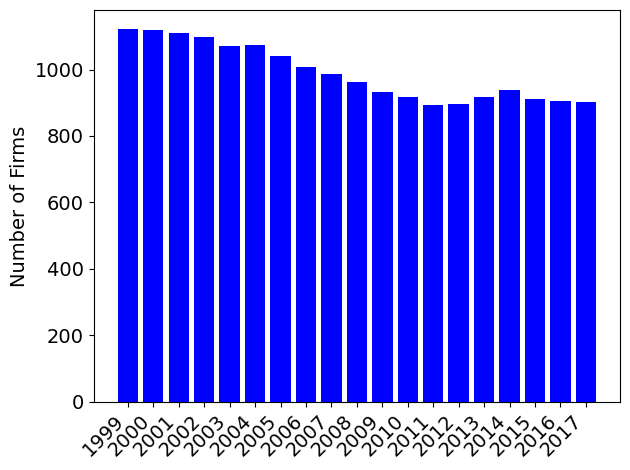
\includegraphics[width=8cm]{figures/number_of_firm}
  \end{center}
\end{frame}

\begin{frame}{Trend of Product Substitutability}
  \begin{center}
    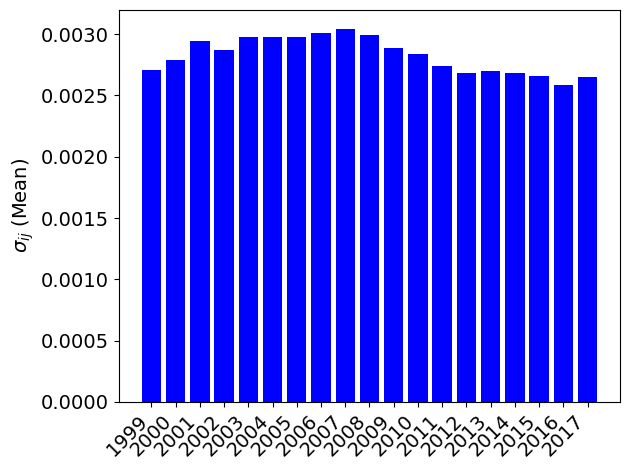
\includegraphics[width=8cm]{figures/sigma}
  \end{center}
\end{frame}

\begin{frame}{Technological Proximity}
  \begin{itemize}
    \item Merge USPTO data with Compustat firms using DISCERN 2 dataset \citep{Arora2024-ad}
    \item Jaffe measure, Group-level patent classification, Stack for 5 years
  \end{itemize}
  \begin{center}
    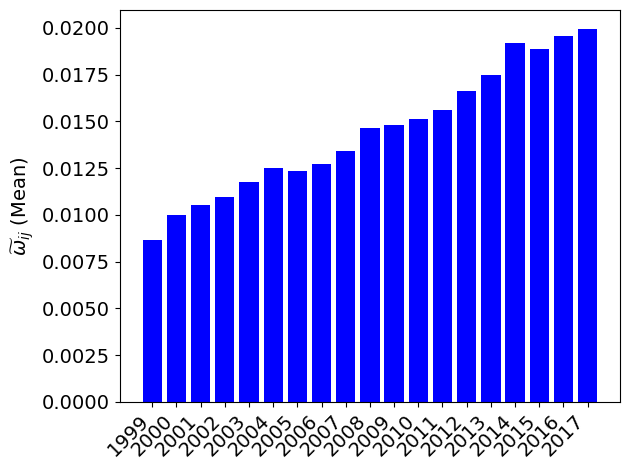
\includegraphics[width=7cm]{figures/omega}
  \end{center}
\end{frame}

\begin{frame}{Distributions of Estimated Knowledge Capital and Quantity}
  \begin{center}
    \begin{figure}
      \centering
      \setcounter{subfigure}{0}
      \subfloat[Log of Quantity]{\begin{centering}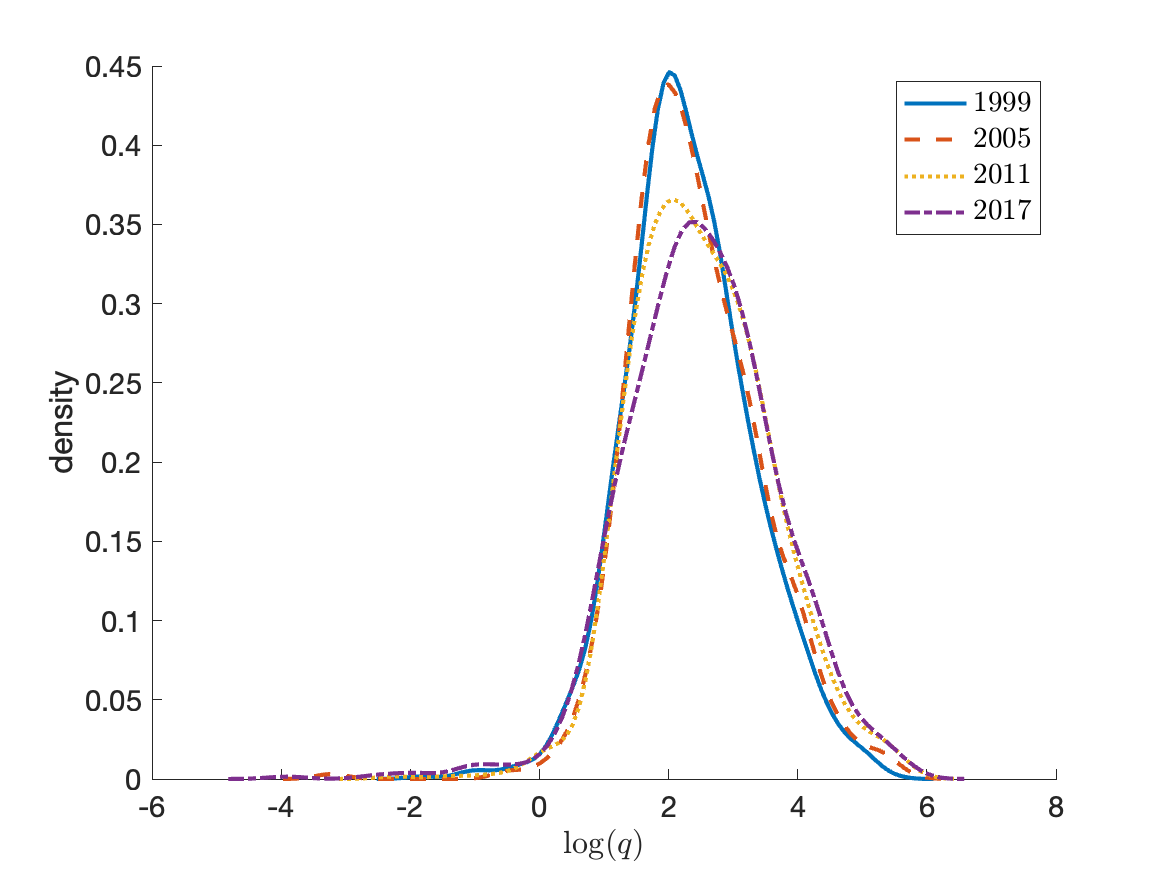
\includegraphics[width=7cm]{figures/log_q_density}\par\end{centering}}
      \subfloat[Log of Knowledge Capital]{\begin{centering}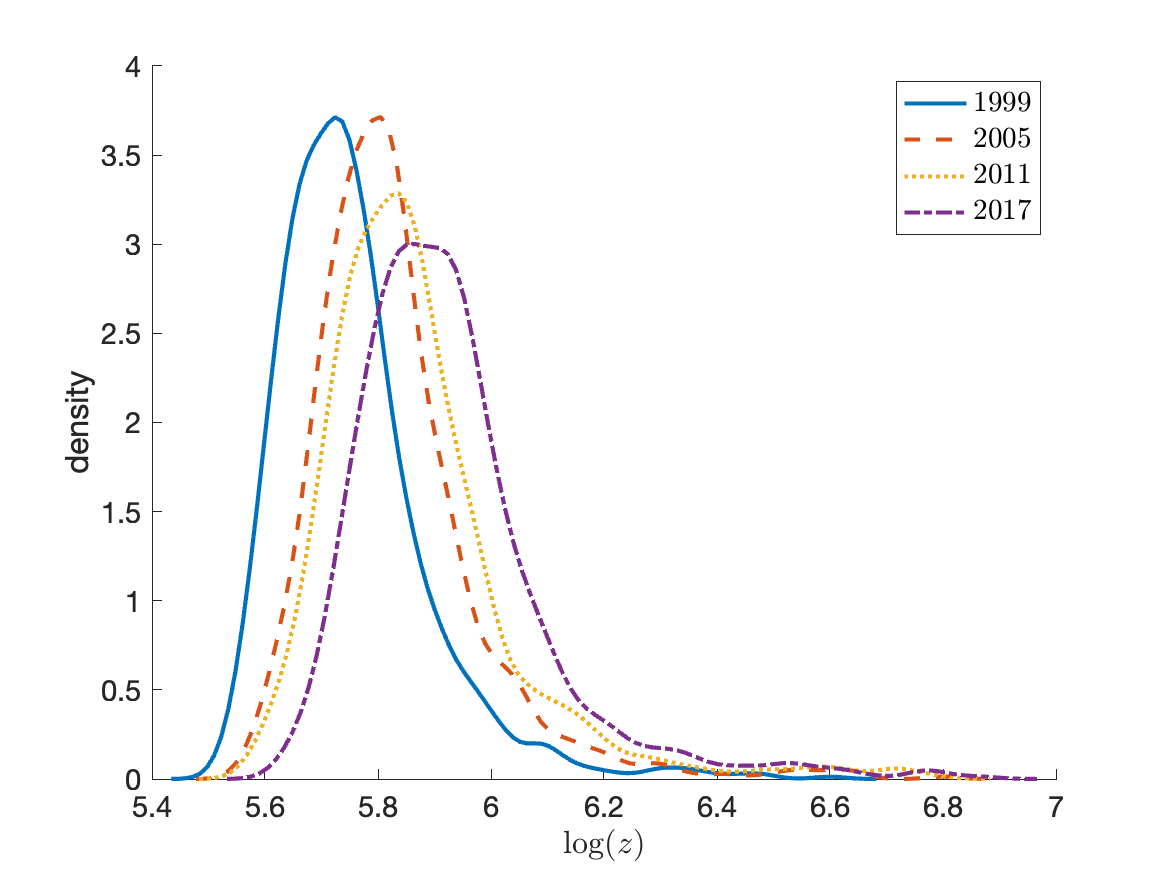
\includegraphics[width=7cm]{figures/log_z_density}\par\end{centering}}
    \end{figure}
  \end{center}
\end{frame}

\begin{frame}[t]{Microeconometric Estimates vs.\ GHL \citep{Pellegrino2024-dn} (1/2)}
  \label{micro_vs_ghl}
  \begin{center}
    \begin{tabular}{lllrr}
      \toprule
      Market      & Firm $i$           & Firm $j$           & \multicolumn{1}{c}{Micro Estimate} & \multicolumn{1}{c}{GHL}    \\
      \midrule
      Auto        & Ford               & Ford               & -4.320         & -5.197 \\
      Auto        & Ford               & General Motors     &  0.034         &  0.056 \\
      Auto        & Ford               & Toyota             &  0.007         &  0.017 \\
      Auto        & General Motors     & Ford               &  0.065         &  0.052 \\
      Auto        & General Motors     & General Motors     & -6.433         & -4.685 \\
      Auto        & General Motors     & Toyota             &  0.008         &  0.005 \\
      Auto        & Toyota             & Ford               &  0.018         &  0.025 \\
      Auto        & Toyota             & General Motors     &  0.008         &  0.008 \\
      Auto        & Toyota             & Toyota             & -3.085         & -4.851 \\
      \bottomrule
    \end{tabular}
  \end{center}
  \hyperlink{product_identification}{\beamerbutton{Back}}
\end{frame}

\begin{frame}[t]{Microeconometric Estimates vs.\ GHL \citep{Pellegrino2024-dn}  (2/2)}
  \begin{center}
    \begin{tabular}{lllrr}
      \toprule
      Market      & Firm $i$           & Firm $j$           & Micro Estimate & GHL    \\
      \midrule
      Cereals     & Kellogg's          & Kellogg's          & -3.231         & -1.770 \\
      Cereals     & Kellogg's          & Quaker Oats        &  0.033         &  0.023 \\
      Cereals     & Quaker Oats        & Kellogg's          &  0.046         &  0.031 \\
      Cereals     & Quaker Oats        & Quaker Oats        & -3.031         & -1.941 \\
      \addlinespace
      Computers   & Apple              & Apple              & -11.979        & -8.945 \\
      Computers   & Apple              & Dell               &  0.018         &  0.025 \\
      Computers   & Dell               & Apple              &  0.027         &  0.047 \\
      Computers   & Dell               & Dell               & -5.570         & -5.110 \\
      \bottomrule
    \end{tabular}
  \end{center}
  \hyperlink{product_identification}{\beamerbutton{Back}}
\end{frame}

\begin{frame}{First Stage \hyperlink{regression}{\beamerbutton{Back}}}
  \label{first_stage}
  \begin{center}
    \begin{tabular}{cc}
      \hline
      \hline              & (1)\tabularnewline
      Dependent Variable: & $\text{\ensuremath{z_{i,t}}}$\tabularnewline
      \hline
      User cost of R\&D   & $\begin{array}{c}
      -39.495^{***} \\
      (4.7044)
      \end{array}$\tabularnewline
      \hline
      Year Fixed Effects  & $\checkmark$\tabularnewline
      No. observations    & 12,947\tabularnewline
      \hline
    \end{tabular}
    \medskip{}
  \end{center}
  {\footnotesize
  SEs clustered by years and 4-digit NAICS industries are reported in parentheses.
  }
  \medskip{}
  \begin{itemize}
    \item IV: User cost of R\&D, driven by state-level tax variations \citep{Wilson2009-ri,Bloom2013-pn}
  \end{itemize}
\end{frame}

\begin{frame}{Alternative Corporate Governance Models: \\ \citet{Ederer2024-rw}}
  \begin{enumerate}
    \item Super-proportional influence: $\tilde{\kappa}_{ij}=\frac{\sum_{z=1}^{Z}s_{iz}\gamma_{iz}s_{jz}}{\sum_{z=1}^{Z}s_{iz}\gamma_{iz}s_{iz}}$ where $\gamma_{iz}=\sqrt{s_{iz}}$
    \medskip{}
    \item Blockholder influence: $\tilde{\kappa}_{ij}=\frac{\sum_{z=1}^{Z}s_{iz}b_{iz}s_{jz}}{\sum_{z=1}^{Z}s_{iz}s_{jz}}\quad(i\neq j),$ where $b_{iz}=1$ if $s_{iz}>5\%$
    \medskip{}
    \item Governance frictions and entrenchment
    \begin{itemize}
      \item \citet{Azar2021-mb} (AR) estimate an objective function where the manager of firm $i$ discounts other firms' profit by $\tau_{i}$
    \end{itemize}
  \end{enumerate}
\end{frame}

\begin{frame}{Alternative Corporate Governance Models}
  \footnotesize
  \begin{tabular}{@{}lcccccc@{}}
    \toprule
    & \multicolumn{6}{c}{Ownership Structure in 2017} \\
    \midrule
    & \shortstack{Dispersed \\ Ownership}
    & \shortstack{Baseline: \\ Proportional \\ Influence}
    & \shortstack{Super \\ Proportional \\ Influence}
    & \shortstack{Blockholder \\ Influence}
    & \shortstack{Governance \\ Frictions \\ (Uniform)}
    & \shortstack{Governance \\ Frictions \\ (Firm-Specific)} \\
    \midrule
    \shortstack[l]{Total Output}
    & 100.00 & 97.57 & 97.36 & 98.25 & 99.31 & 99.49 \\
    \shortstack[l]{Total R\&D Expenditure}
    & 100.00 & 85.73 & 84.48 & 91.05 & 97.57 & 98.70 \\
    \shortstack[l]{Expected Growth Rate (\%) }
    & 1.796 & 1.753 & 1.750 & 1.771 & 1.788 & 1.791 \\
    \shortstack[l]{Expected Social Welfare}
    & 100.00 & 97.18 & 96.94 & 98.01 & 99.21 & 99.41 \\
    \shortstack[l]{Firm Value Share (\%) }
    & 28.74 & 34.32 & 34.32 & 32.79 & 30.65 & 30.78 \\
    \bottomrule
\end{tabular}
\end{frame}

\bibliographystyle{econ-aea}
\bibliography{bibtex}

\end{document}